%==============================================================================
% queues-performance.tex
%==============================================================================

\chapter{Performance Evaluation}
\label{chap:queues-performance}

We evaluate the performance of the different work-stealing queue
implementations when used by the intervals scheduler with a variety of
parallel Java Grande Forum benchmarks (Appendix \ref{chap:benchmarks})
on two different machines:

\begin{itemize}
\item Intel Core2 Duo with one processor and two cores, running Ubuntu
  10.04 64-bit with kernel 2.6.32 and Sun Hotspot JDK 1.6.0\_20
  (Appendix \ref{sec:experimental-setup-marvin})
\item Intel Nehalem with two processors and eight cores, running
  Ubuntu 9.04 64-bit with kernel 2.6.29 and Sun Hotspot JDK 1.6.0\_20
  (Appendix \ref{sec:experimental-setup-mafushi})
\end{itemize}

Both machines invoke the JVM with the following parameters:

\begin{lstlisting}[style=Listing]
  -server -Xmx2048M -Xms2048M -Xss8m
\end{lstlisting}

The execution time reported is the average of the 3 best benchmark
iterations from 10 separate invocations.


\section{Intervals}
\label{sec:queues-performance-intervals}

The performance of the intervals implementation of the JGF benchmarks
is comparable to the threaded implementation (Figure
\ref{fig:queues-performance-threads}).

\begin{figure}[!ht]
  \centering
  \subfloat[Results for the Intel Core2 Duo machine]{
    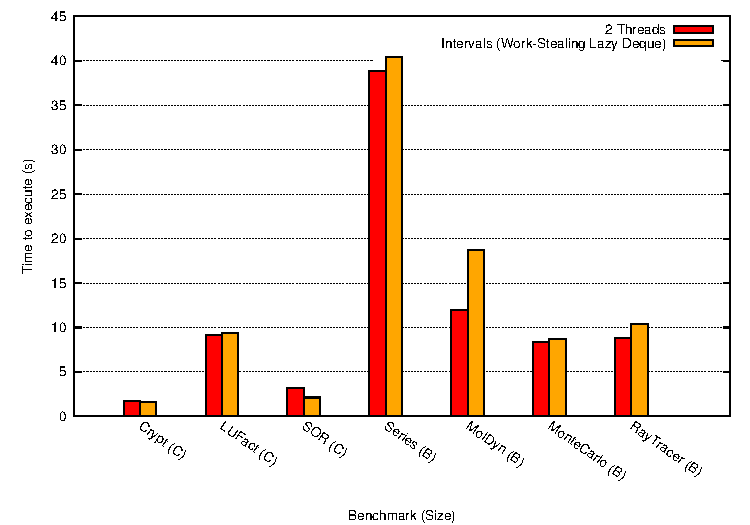
\includegraphics[width=0.89\linewidth]{queues-performance/marvin-threads}
    \label{fig:queues-performance-marvin-threads}
  }
  \\
  \subfloat[Results for the Intel Nehalem machine]{
    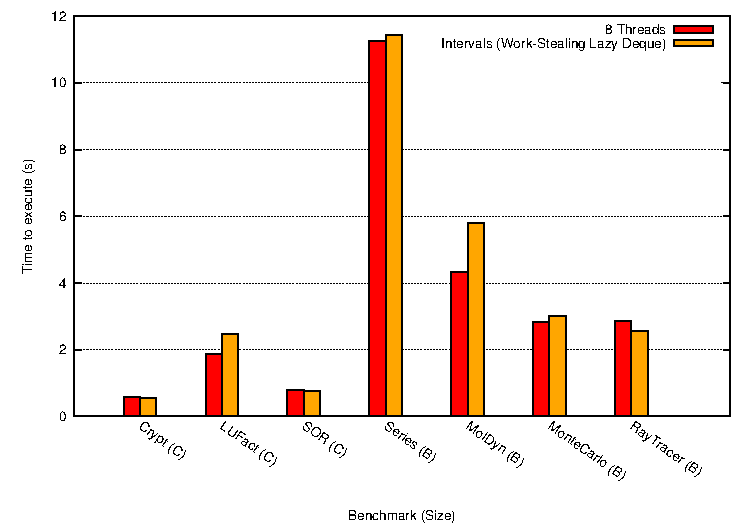
\includegraphics[width=0.89\linewidth]{queues-performance/mafushi-threads}
    \label{fig:queues-performance-mafushi-threads}
  }
  \caption[Threads and intervals benchmarks]{Threads and intervals
    benchmarks running on our Intel Core2 Duo (Appendix
    \ref{sec:experimental-setup-marvin}) and Intel Nehalem (Appendix
    \ref{sec:experimental-setup-mafushi}) test machines}
  \label{fig:queues-performance-threads}
\end{figure}

The only benchmarks where intervals are considerably slower than
threads are \emph{LuFact} and \emph{MolDyn}. The main reason is that
the way work is distributed between intervals makes the workers run
out of work too often. When a worker runs out of work, it becomes idle
and only wakes up if a new work item is added to its queue. Idle
workers acquire a local semaphore which blocks until release is
invoked by some other worker and are added to a global idle list
guarded by a shared lock. If there is an idle worker, adding a new
work item releases the semaphore of the worker and removes it from the
idle list.

Putting a worker to sleep and waking it up again is quite
expensive. Compared to other benchmarks, workers in \emph{LuFact} and
\emph{MolDyn} run out of work more often (Table
\ref{tab:queues-performance-threads}).

\begin{table}[htb]
  \centering
  \subfloat[Results for the Intel Core2 Duo machine]{
    \begin{tabular}{l*{5}{c}}
      \toprule
      & \emph{LuFact} (C) & \emph{MolDyn} (B) & \emph{Crypt} (C) & \emph{SOR} (C) & \emph{RayTracer} (B) \\\midrule
      Idle & \numprint{3533} & \numprint{271} & \numprint{9} & \numprint{6} & \numprint{6} \\
      Woke up\hspace{0.2cm} & \numprint{3531} & \numprint{269} & \numprint{7} & \numprint{4} & \numprint{4} \\\bottomrule
    \end{tabular}
    \label{tab:queues-performance-marvin-threads}
  }
  \\[10ex]
  \subfloat[Results for the Intel Nehalem machine]{
    \begin{tabular}{l*{5}{c}}
      \toprule
      & \emph{LuFact} (C) & \emph{MolDyn} (B) & \emph{Crypt} (C) & \emph{SOR} (C) & \emph{RayTracer} (B) \\\midrule
      Idle & \numprint{11226} & \numprint{1057} & \numprint{27} & \numprint{22} & \numprint{17} \\
      Woke up\hspace{0.2cm} & \numprint{11218} & \numprint{1051} & \numprint{19} & \numprint{14} & \numprint{9} \\\bottomrule
    \end{tabular}
    \label{tab:queues-performance-mafushi-threads}
  }
  \\[2ex]
  \caption{Number of times workers run out of work, become idle, and get woken up again}
  \label{tab:queues-performance-threads}
\end{table}


\section{Work-Stealing Queues}
\label{sec:queues-performance-ws}

When comparing our implementations of the work-stealing queue,
\emph{Work-Stealing Deque} (Section
\ref{sec:queues-implementation-ws-deque}) and \emph{Idempotent
  Work-Stealing Deque} (Section
\ref{sec:queues-implementation-idempotent-ws-deque}), with the
original \emph{Work-Stealing Lazy Deque} (Section
\ref{sec:queues-background-current-implementation}) we do not see a
significant difference in the runtime of the JGF benchmarks (Figure
\ref{fig:queues-performance-deques}) on both machines we tested them
on.

The reason for this is that the \emph{Work-Stealing Lazy Deque}
implementation is very efficient already. Using a lock in the
\lstinline!steal()! method is of less impact than we thought it would
be.

The \emph{Work-Stealing Lazy Deque} uses an
\lstinline!AtomicReferenceArray! to maintain work items. The
\lstinline!AtomicReferenceArray! provides volatile access semantics
for its array elements, which is not supported for ordinary
arrays. Because of this, \emph{Work-Stealing Lazy Deque} does not have
to use additional volatile or atomic variables like the other deque
implementations do. This allows for a simpler implementation.

The location of the head of the \emph{Work-Stealing Lazy Deque} is
only lazily updated by its owner. This means the location of the head
is only updated when its owner tries to take a work item and finds it
was stolen by a competing thief -- as opposed to the methods
\lstinline!take()! and \lstinline!steal()!  of the \emph{Work-Stealing
  Deque} which attempt to update the location of the head on every
execution with a Compare-and-Swap operation. Similarly the methods
\lstinline!take()!  and \lstinline!steal()! of the \emph{Idempotent
  Work-Stealing Deque} have to update the size in the anchor on every
execution.

Another reason for the lack of difference between the queue
implementations might be the small number of cores of the systems we
had to test them on. See Section
\ref{sec:queues-performance-single-shared-queue} for more details.

\begin{figure}[!ht]
  \centering
  \subfloat[Results for the Intel Core2 Duo machine]{
    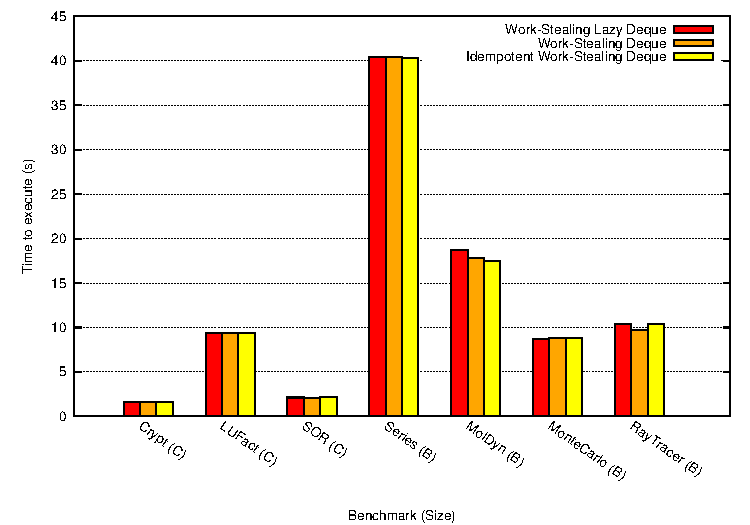
\includegraphics[width=0.89\linewidth]{queues-performance/marvin-deques}
    \label{fig:queues-performance-marvin-deques}
  }
  \\
  \subfloat[Results for the Intel Nehalem machine]{
    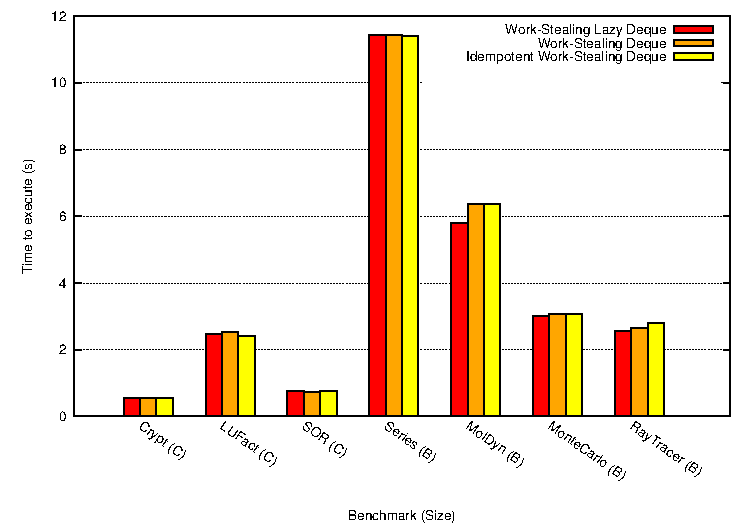
\includegraphics[width=0.89\linewidth]{queues-performance/mafushi-deques}
    \label{fig:queues-performance-mafushi-deques}
  }
  \caption[Work-stealing deques benchmarks]{Work-stealing deques
    benchmarks running on Intel Core2 Duo (Appendix
    \ref{sec:experimental-setup-marvin}) and Intel Nehalem (Appendix
    \ref{sec:experimental-setup-mafushi})}
  \label{fig:queues-performance-deques}
\end{figure}


\section{Alternative Work-Stealing Queues}
\label{sec:queues-performance-alternative}

\subsection{Dynamic Work-Stealing Deque}
\label{sec:queues-performance-alternative-dynamic}

The implementation of the \emph{Dynamic Work-Stealing Deque} (Section
\ref{sec:queues-alternative-implementations-dynamic-deque}) requires
extra work for the list's maintenance which reflects in its
performance: Most of the benchmarks are slightly slower in comparison
to other queue implementations. Figure
\ref{fig:queues-performance-dynamic} shows the benchmark runtimes of
the \emph{Dynamic Work-Stealing Deque} in comparison to the
\emph{Work-Stealing Deque}.

% Bug in dynamic work-stealing deque implementation: steal() always
% returns null and never succeeds! This is the reason why benchmarks
% with uneven work item distribution (Series and MonteCarlo) have more
% or less the runtime of the single threaded implementation.

\begin{figure}[!htb]
  \centering
  \subfloat[Results for the Intel Core2 Duo machine]{
    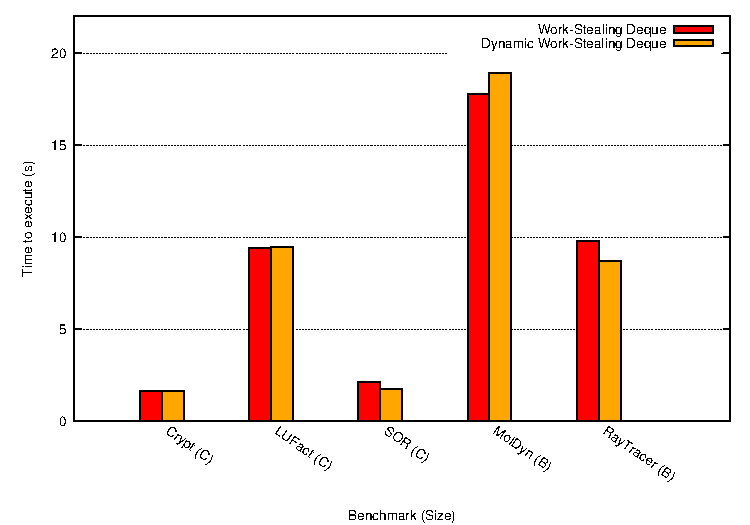
\includegraphics[width=0.5\linewidth]{queues-performance/marvin-dynamic}
    \label{fig:queues-performance-marvin-dynamic}
  }
  \subfloat[Results for the Intel Nehalem machine]{
    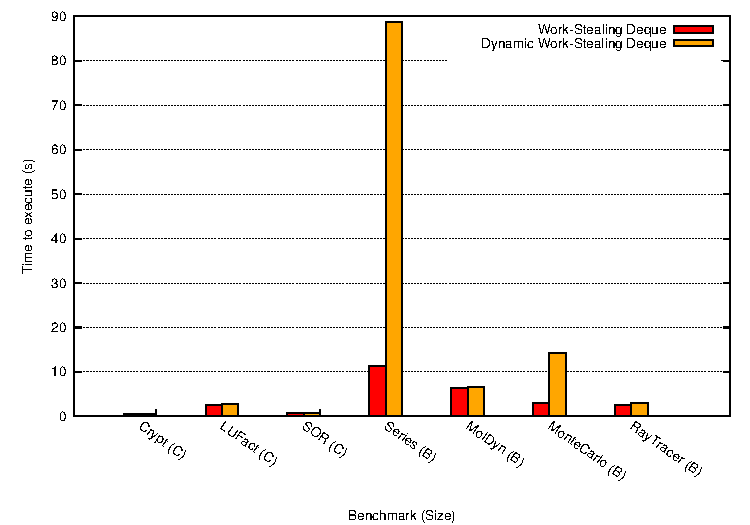
\includegraphics[width=0.5\linewidth]{queues-performance/mafushi-dynamic}
    \label{fig:queues-performance-mafushi-dynamic}
  }
  \caption[Dynamic work-stealing deques benchmarks]{Dynamic
    work-stealing deques benchmarks running on Intel Core2 Duo
    (Appendix \ref{sec:experimental-setup-marvin}) and Intel Nehalem
    (Appendix \ref{sec:experimental-setup-mafushi})}
  \label{fig:queues-performance-dynamic}
\end{figure}

\subsection{Idempotent Work-Stealing Queues}
\label{sec:performance-alternative-idempotent}

When experimenting with idempotent queues, we also implemented the
\emph{Idempotent Work-Stealing FIFO Queue} and \emph{Idempotent
  Work-Stealing LIFO Queue} to compare them to the \emph{Idempotent
  Work-Stealing Deque}. It turned out that the \emph{Idempotent
  Work-Stealing Deque} has the best performance in combination with
the intervals scheduler (Figure
\ref{fig:queues-performance-idempotent}).

The \emph{Idempotent Work-Stealing FIFO Queue} behaves like a normal
queue: \lstinline!put()! puts tasks at the tail, and
\lstinline!take()!  and \lstinline!steal()! remove tasks at the
head. As \lstinline!take()! and \lstinline!steal()! work on the same
end of the queue, they have to deal with increased contention. This
often reflects itself in a lower performance due to a higher number of
take and steal failures in the \emph{Idempotent Work-Stealing FIFO
  Queue} compared to the \emph{Idempotent Work-Stealing Deque} (Table
\ref{tab:queues-performance-idempotent-fifo}). This is especially
visible in the runtimes of the \emph{SOR} and \emph{MolDyn} benchmarks
(Figure \ref{fig:queues-performance-idempotent}). In the
\emph{Idempotent Work-Stealing Deque} there is less contention between
\lstinline!take()! and \lstinline!steal()! as they work on opposite
ends of the queue.

\begin{figure}[!htb]
  \centering
  \subfloat[Results for the Intel Core2 Duo machine]{
    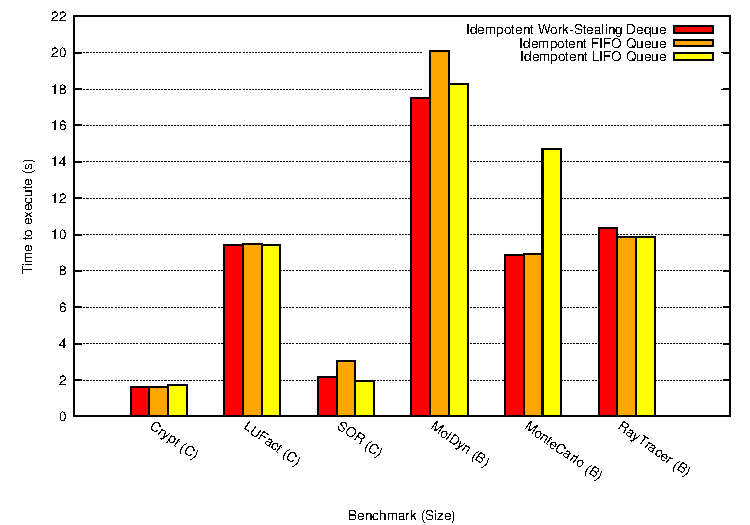
\includegraphics[width=0.89\linewidth]{queues-performance/marvin-idempotent}
    \label{fig:queues-performance-marvin-idempotent}
  }
  \\
  \subfloat[Results for the Intel Nehalem machine]{
    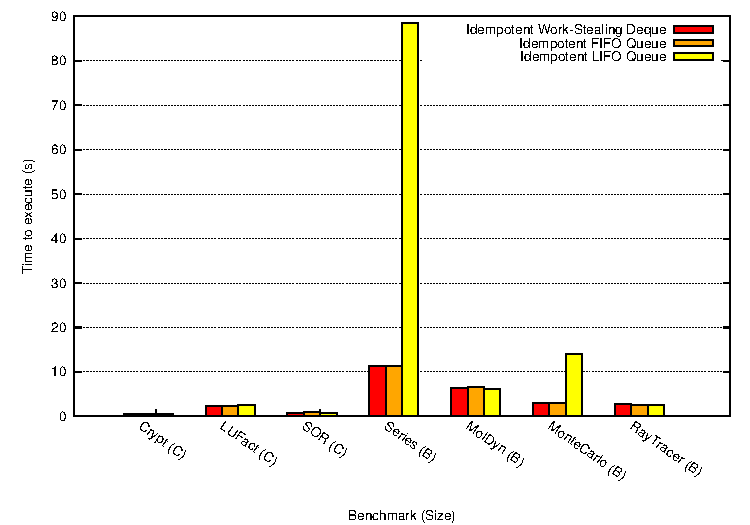
\includegraphics[width=0.89\linewidth]{queues-performance/mafushi-idempotent}
    \label{fig:queues-performance-mafushi-idempotent}
  }
  \caption[Idempotent work-stealing queues benchmarks]{Idempotent
    work-stealing queues benchmarks running on Intel Core2 Duo
    (Appendix \ref{sec:experimental-setup-marvin}) and Intel Nehalem
    (Appendix \ref{sec:experimental-setup-mafushi})}
  \label{fig:queues-performance-idempotent}
\end{figure}

\begin{table}[!htb]
  \centering
  \subfloat[Results for the Intel Core2 Duo machine]{
   \begin{tabular}{lrrrr}
     & \multicolumn{2}{c}{\hspace{0.5cm}\emph{SOR} (C)} & \multicolumn{2}{c}{\hspace{0.5cm}\emph{MolDyn} (B)} \\
     & \hspace{0.5cm}Deque & \hspace{0.5cm}Queue & \hspace{1cm}Deque & \hspace{0.5cm}Queue \\
     \toprule
     Take Attempts & \numprint{149937} & \numprint{150021} & \numprint{3662} & \numprint{3667} \\
     Take Failures & \numprint{504} & \numprint{27450} & \numprint{607} & \numprint{673} \\
     \midrule
     Steal Attempts & \numprint{650} & \numprint{27684} & \numprint{615} & \numprint{673} \\
     Steal Failures & \numprint{153} & \numprint{238} & \numprint{265} & \numprint{266} \\
     \bottomrule
   \end{tabular}
    \label{tab:queues-performance-marvin-idempotent-fifo}
  }
  \\[5ex]
  \subfloat[Results for the Intel Nehalem machine]{
    \begin{tabular}{lrrrr}
      & \multicolumn{2}{c}{\hspace{0.5cm}\emph{SOR} (C)} & \multicolumn{2}{c}{\hspace{0.5cm}\emph{MolDyn} (B)} \\
      & \hspace{0.5cm}Deque & \hspace{0.5cm}Queue & \hspace{1cm}Deque & \hspace{0.5cm}Queue \\
      \toprule
      Take Attempts & \numprint{150051} & \numprint{150118} & \numprint{14197} & \numprint{14076} \\
      Take Failures & \numprint{2108} & \numprint{16293} & \numprint{3327} & \numprint{4421} \\
      \midrule
      Steal Attempts & \numprint{4778} & \numprint{34190} &\numprint{12742} & \numprint{15095} \\
      Steal Failures & \numprint{2734} & \numprint{17930} & \numprint{10490} & \numprint{11718} \\
      \bottomrule
    \end{tabular}
    \label{tab:queues-performance-mafushi-idempotent-fifo}
  }
  \caption{Comparing take and steal attempts and failures of the \emph{Idempotent Work-Stealing Deque} with the \emph{Idempotent Work-Stealing FIFO Queue}}
  \label{tab:queues-performance-idempotent-fifo}
\end{table}

\begin{table}[!htb]
  \centering
  \subfloat[Results for the Intel Core2 Duo machine]{
    \begin{tabular}{lrrrr}
      & \multicolumn{2}{c}{\hspace{0.5cm}\emph{Series} (C)} & \multicolumn{2}{c}{\hspace{0.5cm}\emph{MonteCarlo} (B)} \\
      & \hspace{0.5cm}Deque & \hspace{0.5cm}Stack & \hspace{1cm}Deque & \hspace{0.5cm}Stack \\
      \toprule
      Take Attempts & \numprint{100037} & \numprint{100008} & \numprint{60078} & \numprint{60005} \\
      Take Failures & \numprint{49705} & \numprint{78} & \numprint{29979} & \numprint{41} \\
      \midrule
      Steal Attempts & \numprint{49921} & \numprint{886483626} & \numprint{30257} & \numprint{151331850} \\
      Steal Failures & \numprint{223} & \numprint{886483555} & \numprint{283} & \numprint{151331813} \\
      \bottomrule
    \end{tabular}
    \label{tab:queues-performance-marvin-idempotent-lifo}
  }
  \\[5ex]
  \subfloat[Results for the Intel Nehalem machine]{
    \begin{tabular}{lrrrr}
      & \multicolumn{2}{c}{\hspace{0.5cm}\emph{Series} (C)} & \multicolumn{2}{c}{\hspace{0.5cm}\emph{MonteCarlo} (B)} \\
      & \hspace{0.5cm}Deque & \hspace{0.5cm}Stack & \hspace{1cm}Deque & \hspace{0.5cm}Stack \\
      \toprule
      Take Attempts & \numprint{101446} & \numprint{100049} & \numprint{61989} & \numprint{60017} \\
      Take Failures & \numprint{88867} & \numprint{175} & \numprint{54333} & \numprint{125} \\
      \midrule
      Steal Attempts & \numprint{391742} & \numprint{436934995} & \numprint{244771} & \numprint{71468669} \\
      Steal Failures & \numprint{302891} & \numprint{436934868} & \numprint{190454} & \numprint{71468560} \\
      \bottomrule
    \end{tabular}
    \label{tab:queues-performance-mafushi-idempotent-lifo}
  }
  \caption{Comparing take and steal attempts and failures of the \emph{Idempotent Work-Stealing Deque} with the \emph{Idempotent Work-Stealing LIFO Queue}}
  \label{tab:queues-performance-idempotent-lifo}
\end{table}

The \emph{Idempotent Work-Stealing LIFO Queue} behaves like a stack:
\lstinline!put()! puts tasks at the tail, and \lstinline!take()!  and
\lstinline!steal()! remove tasks at the tail too. As
\lstinline!put()!, \lstinline!take()! and \lstinline!steal()! work on
the same end of the queue, they have to deal with increased
contention. This especially shows in the performance of the
\emph{Series} and \emph{MonteCarlo} benchmarks with an extremely high
number of steal attempts and failures compared to the \emph{Idempotent
  Work-Stealing Deque} (Table
\ref{tab:queues-performance-idempotent-lifo}).

\subsection{Duplicating Work-Stealing Queue}
\label{sec:performance-alternative-duplicating}

We implemented the \emph{Duplicating Work-Stealing Queue} (Section
\ref{sec:queues-alternative-implementations-duplicating-queue}) as an
alternative to the \emph{Idempotent Work-Stealing Deque}. Both use
idempotent intervals, but whereas the idempotent work-stealing deque
relies on atomic Compare-and-Swap operations and uses a tag to prevent
the ABA problem, the duplicating work-stealing queue uses a lock on
all but the critical paths. Despite the usage of locks in the
duplicating work-stealing queue we could not find any significant
performance difference to the idempotent work-stealing deque (Figure
\ref{fig:queues-performance-duplicating}).

\begin{figure}[!htb]
  \centering
  \subfloat[Results for the Intel Core2 Duo machine]{
    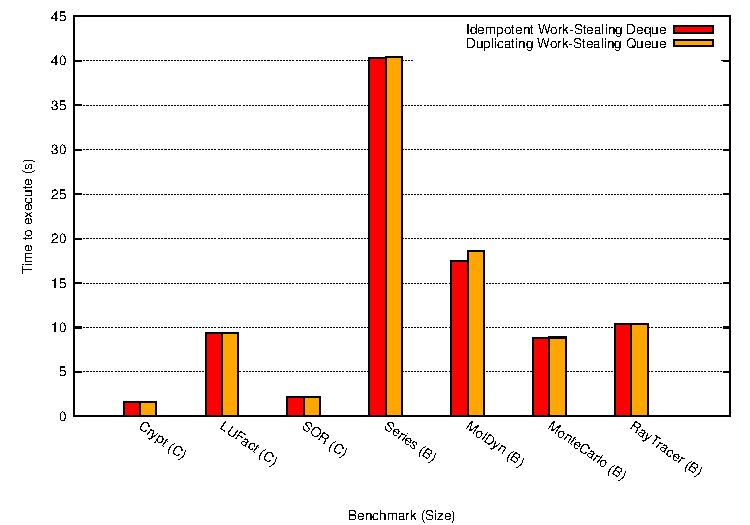
\includegraphics[width=0.5\linewidth]{queues-performance/marvin-duplicating}
    \label{fig:queues-performance-marvin-duplicating}
  }
  \subfloat[Results for the Intel Nehalem machine]{
    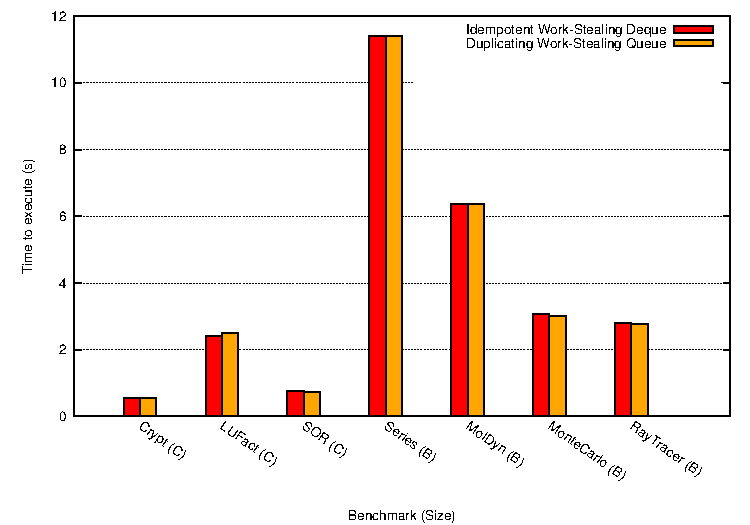
\includegraphics[width=0.5\linewidth]{queues-performance/mafushi-duplicating}
    \label{fig:queues-performance-mafushi-duplicating}
  }
  \caption[Duplicating benchmarks]{Duplicating benchmarks running on
    Intel Core2 Duo (Appendix \ref{sec:experimental-setup-marvin}) and
    Intel Nehalem (Appendix \ref{sec:experimental-setup-mafushi})}
  \label{fig:queues-performance-duplicating}
\end{figure}


\section{Single Shared Work Queue}
\label{sec:queues-performance-single-shared-queue}

None of the work-stealing queues we developed significantly improves
work-stealing performance (Section \ref{sec:queues-performance-ws}) on
the machines we had to test them with (Appendix
\ref{chap:experimental-setup}). \textcite{Saha2007} state that there
is no noticeable difference between the speedup of work-stealing and a
global shared work queue when not using more than 8 cores. If this is
the case, then the optimizations we did in our work-stealing queue
implementations most likely will not have any significant effect
either.

To check this hypothesis, we rewrote the intervals scheduler to use a
single shared work deque. The shared work deque is implemented with
\lstinline!LinkedBlockingDeque! from the
\lstinline!java.util.concurrent! package in a stack-like manner: Items
are added with \lstinline!addLast()! at the end of the queue and taken
with \lstinline!pollLast()! from the end of the queue. For comparison
we added another work-stealing implementation changing the original
intervals scheduler to use \lstinline!LinkedBlockingDeque!.

Our experiments confirm the hypothesis for the JGF benchmarks. There
is no significant difference between the runtimes of the different
implementations: Whether we use work-stealing with the
\emph{Work-Stealing Deque} or the \emph{Linked Blocking Deque}, or the
\emph{Single Shared Work Queue} instead of work-stealing, we get
almost the same results (Figure
\ref{fig:queues-performance-shared-queue}).

\begin{figure}[!ht]
  \centering
  \subfloat[Results for the Intel Core2 Duo machine]{
    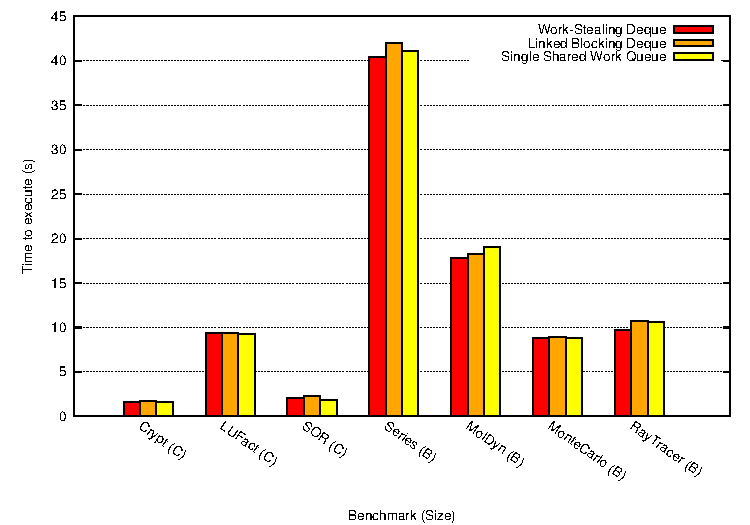
\includegraphics[width=0.68\linewidth]{queues-performance/marvin-shared-queue}
    \label{fig:queues-performance-marvin-shared-queue}
  }
  \\
  \subfloat[Results for the Intel Nehalem machine]{
    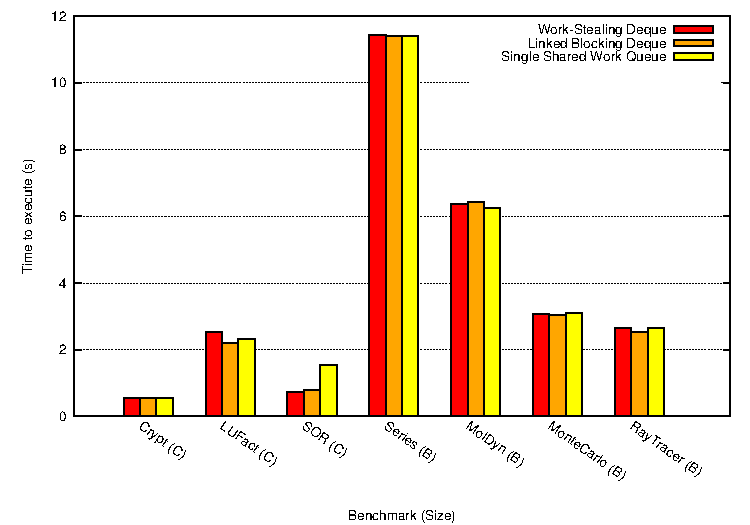
\includegraphics[width=0.68\linewidth]{queues-performance/mafushi-shared-queue}
    \label{fig:queues-performance-mafushi-shared-queue}
  }
  \caption[Shared queue benchmarks]{Shared queue benchmarks running on
    Intel Core2 Duo (Appendix \ref{sec:experimental-setup-marvin}) and
    Intel Nehalem (Appendix \ref{sec:experimental-setup-mafushi})}
  \label{fig:queues-performance-shared-queue}
\end{figure}

To really study the impact of work-stealing queues on the intervals
implementation, we need to do extend our experiments to machines with
more than 8 cores.


%%% Local Variables: 
%%% mode: latex
%%% TeX-master: "thesis"
%%% End: 
